\documentclass{beamer}
\usepackage[utf8]{inputenc}
\usepackage{amsmath, amsfonts, epsfig, xspace}
%\usepackage{algorithm,algorithmic}
\usepackage{pstricks,pst-node}
%\usepackage{movie15} % multimedia, movie15
\usepackage[movieson]{optional}
\usepackage[normal,tight,center]{subfigure}
\usepackage{booktabs} % book-quality tables
\usepackage{fancybox}

\usepackage[utf8]{inputenc}
\usepackage{amssymb}

% PRESENTATION LANGUAGE
\usepackage[spanish]{babel}

% BIB
\usepackage{natbib}  
\def\newblock{}

% DEFINITION OF UPC BLUE
\definecolor{upcblue}{rgb}{0.262745098,0.556862745,0.77254902}
\definecolor{MainBlue}{rgb}{0.2,0.2,0.7}
\definecolor{MainGreen}{RGB}{0, 128, 0}
\definecolor{MainRed}{rgb}{0.73,0.08,0.21}
\definecolor{MyBrickRed}{rgb}{0.549, 0.239, 0.271}    
\definecolor{MyStrongRed}{rgb}{0.60, 0, 0.06}    
\definecolor{MyWebBrown}{rgb}{0.6, 0, 0}
\definecolor{MyWebBlue}{rgb}{0.2, 0.2, 1.0}%{0.07, 0.07, 0.53}

% http://en.wikibooks.org/wiki/LaTeX/Hyperlinks
% http://www.math.uakron.edu/~dpstory/tutorial/pdfmarks/hyper.pdf
\usepackage{hyperref} 
\hypersetup{colorlinks, urlcolor=MainBlue, citecolor=MainBlue, linkcolor=MainBlue} % BrickRed, RoyalBlue

% SUB-FIGURES
\setlength{\subfigcapskip}{-.5em}

% Beamer scheme
\usepackage{beamerthemesplit}
\usetheme{thesis}

% BASIC SCHEMES
%\usecolortheme[named=upcblue]{structure}
%\useinnertheme{rounded}
%\useoutertheme{shadow}

% SOME MINOR COLOR CHANGES
%\setbeamercolor{palette primary}{fg=upcblue,bg=white}
%\setbeamercolor{palette quaternary}{fg=white,bg=upcblue}

%% NEW COMMANDS
\newcommand{\Neurochem}{\textsc{NEUROChem} }
\newcommand{\Comedi}{\textsc{Comedi} }
\newcommand{\UPC}{Universitat Polit\`ecnica de Catalunya}

\newcommand{\R}{\texttt{R} }
\newcommand{\Python}{\texttt{Python} }

\newcommand{\smaller}{\tiny}
\newcommand{\mancite}[1]{{\scriptsize{\textbf{\color{MainGreen}{[#1] }}}}}

\renewcommand{\emph}[1]{{\color{MainBlue}{#1}}}


% GRAPHICS OPTIONS
\setkeys{Gin}{width=1.0\textwidth}
\graphicspath{{figures/}{images/}}

% INDENT
%\usepackage[parfill]{parskip}

% THE BASIC PRESENTATION INFORMATION
\title[\textnormal{Ph.D. Thesis Proposal \hspace{15em} \insertframenumber/\inserttotalframenumber}]{Computing Platform for Bioispired Chemical Gas Sensing}
\subtitle{Ph.D. Thesis Proposal}
\author[\textnormal{Andrey Ziyatdinov}]{Andrey Ziyatdinov}

%\institute{ 
%  { \small Advisor: Dr. Alexandre Perera} \\ \vspace{0.05\linewidth}  SISBIO - CREB - UPC}
\date{29 June, 2011}

% THE LOGO THAT WILL BE USED IN EACH PAGE
%\logo{
%\includegraphics[width=1.25cm]{logos/creb-upc.jpg} \insertframenumber/\inserttotalframenumber
%}

\begin{document}

% THE TITLE FRAME
\begin{frame}[plain]
  % THE HEADER WITH THE UPC AND CREB LOGOS
  \begin{center}
    \begin{tabular}[\textwidth]{lp{1cm}r}
      
\includegraphics[width=1.5cm]{logos/creb.jpg}
      &
      &
      
\includegraphics[width=1.5cm]{logos/upc.jpg}\\
      \texttt{\tiny Centre de Recerca en Enginyeria Biomèdica}
      &
      &
      \texttt{\tiny Universitat Politècnica de Catalunya}
    \end{tabular}
  \end{center}

  \begin{center}
    %\textsc{\LARGE University of Beer}\\[1.5cm]
    \textsc{\Large Ph.D. Thesis Proposal}\\[0.5cm]
    % Title
    %\HRule \\[0.4cm]
    {\huge \emph{Computing Platform for Bioispired Chemical Gas Sensing}}\\[0.4cm]
    %\HRule \\[1.5cm]

    % Author and supervisor
    \begin{minipage}{0.25\textwidth}
    \begin{flushleft} %\large
      Ph.D. Student: \\
      Supervisor: 
    \end{flushleft}
    \end{minipage}
    \begin{minipage}{0.6\textwidth}
    \begin{flushleft} %\large
      Andrey Ziyatdinov \\
      Alexandre Perera Lluna
    \end{flushleft}
    \end{minipage}
    
    \vfill

    % Bottom of the page
    {\large 29 June, 2011}
  \end{center}

  % THE REST OF THE TITLE
  %\maketitle
\end{frame}

\begin{frame}
  \frametitle{Outline}
  \tableofcontents
\end{frame}

% SECTION
\section{Introduction}

% SUB-ECTION
\subsection{An example of breath analysis}

% frame
\begin{frame}
\frametitle{A Story}
\begin{columns}
\column{0.6\textwidth}
The New York Times \\
\href{http://www.nytimes.com/2006/01/17/health/17dog.html}{Dogs Excel on Smell Test to Find Cancer} \\
{\scriptsize By Donald G. McNeil Jr., 2006}

\begin{block}{}
It has trained five dogs to detect lung cancer in the breath of cancer sufferers with 99\% accuracy. \\
\mancite{Pearce et al., 2003}
%{\scriptsize The Pine Street Clinic, CA}
% (tumors contain alkanes and benzene compounds)
\end{block}

Keys to success
\begin{itemize}
  \item Known biomarkers in exhaled human breath
    are volatile organic compounds such as alkanes 
  \item Dogs detect odors in the very low parts-per-billion range
  \item The unique architecture of the olfactory pathway
\end{itemize}  

\column{0.4\textwidth}
\begin{center}
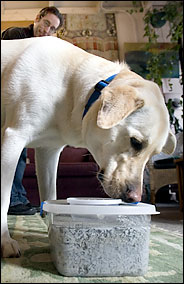
\includegraphics[width=.9\linewidth]{images/dog.jpg} \\
{\tiny Kobi in a cancer-detection experiment}
\end{center}
\end{columns}
\end{frame}

\end{document}



